
\section{Documento de Diseño}

El Documento de Diseño es una herramienta que conduce el desarrollo a lo largo del proyecto y deberá estar dispuesto a sufrir diversos cambios desde la etapa de revisión. Contiene, por escrito, todas las especificaciones necesarias para guiar el proyecto de software. Un documento de diseño tiene que ser una referencia estable, detallando todas las partes del software y cómo van a trabajar.

En metodología ágil será necesario utilizar el product backlog como una verdadera guía para el diseño, este se refinará a lo largo del proyecto, principalmente al finalizar cada sprint.

El Product Backlog o Pila de producto, es un documento donde figuran todas las User Stories (US) capturadas con sus respectivas prioridades, estimaciones y definiciones que definen el  trabajo a realizar (PBI, Product Backlog Item).
Representa todo aquello que esperan los clientes,usuarios, y en general los interesados.

Los elementos del Product Backlog que forman parte del sprint se determinaron durante la reunión de Sprint Planning y fueron detallados en el apartado anterior como objetivos preliminares, en esta sección se presentará como una tabla donde se detallará la prioridad que se le dará a cada una de las user story.

En la \textbf{Figura \ref{scrum}} podemos ver con claridad como a partir de un Product Backlog ordenado según la prioridad, se desprende el backlog del sprint que indica la lista de tareas en las que se han descompuesto las funcionalidades que se van a desarrollar en un sprint. 

En cada tarea del sprint backlog se indicará la persona que tiene asignada dicha tarea y el tiempo de trabajo previsto. También se puede observar que durante el sprint se actualizarán a diario los tiempos pendientes de cada una y que al finalizarlo se obtendrá un producto completamente terminado y probado.
\begin{figure}[h]
  \centering
  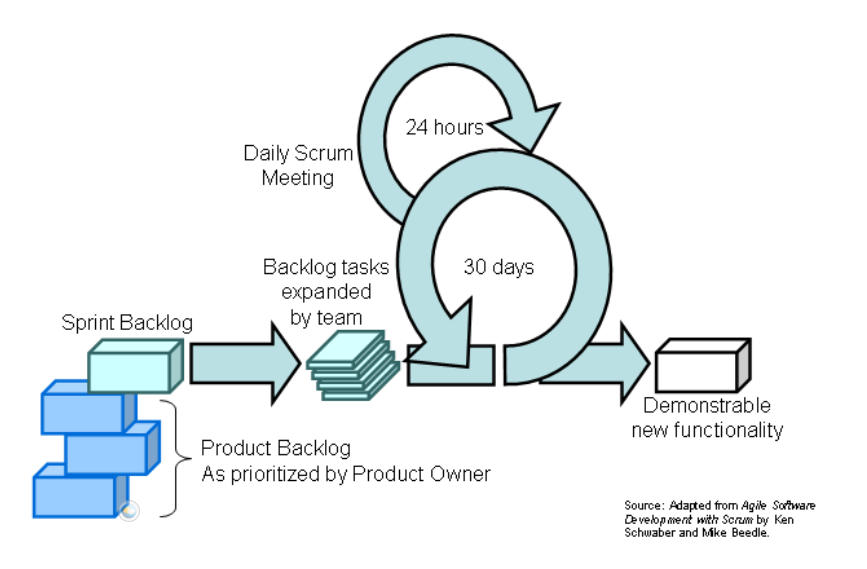
\includegraphics[width=.8\textwidth]{img/tp1_parte2/scrum}
  \caption{Modelo de Trabajo Scrum}
  \label{scrum}
\end{figure}

El producto resultado de un Sprint es el incremento. El incremento tiene como característica que todas las tereas está completamente terminadas y operativas, es decir, en condiciones de ser  entregadas  al cliente. Se detallarán estos resultados en cada uno de los sprint.

No se considerará como incrementos: prototipos, módulos o subrutinas pendientes de pruebas o de integración. Se hará una excepción el primer sprint en el cual se definirán los detalles generales de las tecnologías a utilizar.

\subsection{Product Backlog}

Como se detalló anteriormente, en el product backlog  se recogerán los requerimientos del sistema\/necesidades de los clientes, sobre estos requerimientos se realizará una estimación de tiempo necesario para concretarlo, se establecerán prioridades entre los user stories y finalmente se indicará un comentario para el mismo siempre que sea pertinente. 
En la siguiente \textbf{Tabla} podemos apreciar el product backlog del proyecto.
Se recuerda que estos requerimientos representan una primera aproximación a los requerimientos definitivos por lo que no puede considerarse que están establecidas todas y cada una de las características que el producto tendrá finalmente. Estos serán actualizados y refinados constantemente con el paso del tiempo.


{\scriptsize
\begin{tablaUSNumerada}
	\hline
        \multicolumn{1}{|c|}{\textbf{ID}} &
        \multicolumn{1}{|c|}{\textbf{Enunciado de la historia}} &
        \textbf{Prioridad} \\
	\hline
    \endhead
    
    \hline
        \label{infoPerfil} &
        Como paciente, quiero  añadir información de mi perfil de salud o mediciones regulares para que el médico cuente con más y mejor información al momento de realizar el diagnóstico. 
        & 10 de 10
        
        \\
    \hline
        \label{evitarPerdidas} &
        Como paciente, quiero  añadir al sistema mis estudios realizados para evitar posibles pérdidas. 
        & 9 de 10
        
        \\
    \hline
        \label{infoSalud} &
        Como paciente quiero cargar mi información personal de salud referido a mediciones (altura, grasa corporal, peso, presión arterial), para que el médico cuente con más y mejor información al momento de realizar el diagnóstico. 
        & 10 de 10
        
        \\
    \hline
        \label{diagnosticarPaciente} &
        Como médico quiero diagnosticar a un paciente, para darle un cierre a una incidencia planteada por la persona. 
        &7 de 10
        
        \\
    \hline
        \label{cargaCentroSalud} &
        Como paciente, quiero que los sistemas de salud existentes puedan cargar sus resultados directamente en mi carpeta de salud para centralizar mi información. 
        & 7 de 10
        
        \\
    \hline
        \label{asociarDispositivo} &
        Como paciente, quiero asociar un dispositivo para agilizar y ampliar la carga de datos. 
        &4 de 10
        
        \\
    \hline
        \label{categorizarEstudios} &
        Como paciente, quiero categorizar mis estudios por rama de medicina, para lograr una mejor organización y navegabilidad en el sistema. 
        &7 de 10
        
        \\
    \hline
        \label{infoPaciente} &
        Como laboratorio, quiero cargar información de un paciente en su cuenta para ahorrarle las molestias de volver. 
        & 7 de 10
        
        \\
    \hline
        \label{guardarInfoLocal} &
        Como paciente, quiero guardar mi información de manera local para tener un respaldo. 
        &8 de 10
        
        \\
    \hline
        \label{agregarGrupoFamiliar} &
        Como paciente, quiero agregar personas a mi grupo familiar para llevar el seguimiento de los mismos. 
        &8 de 10
        
        \\
    \hline
        \label{modificarPermisos} &
        Como paciente, quiero modificar los permisos de visualización de mis datos con respecto a cada uno de los integrantes de grupo familiar para tener un control total sobre mi privacidad. 
        &4 de 10
        
        \\
    \hline
        \label{comunicarResultado} &
        Como paciente quiero que no sea necesario ir al hospital para que un medico me comunique los resultados del análisis. 
        & 5 de 10
        
        \\
    \hline
        \label{registrarConFacebook} &
        Como usuario quiero registrarme con una cuenta de Facebook y/o Google para facilitar la inscripción al sitio y el manejo de credenciales. 
        &4 de 10
        
        \\
    \hline
        \label{infoHijo} &
        Como mujer embarazada quiero llevar la información de mi hijo para transmitírsela cuando nazca. 
        &2 de 10
        
        \\
    \hline
        \label{graficaParaMedico} &
        Como médico quiero ver gráficas que resuman la información de un paciente para poder ver sus cambios a lo largo de la historia y así apoyar la toma de decisiones y el diagnóstico. 
        &6 de 10
        
        \\
    \hline
        \label{accesoCualquierLugar} &
        Como paciente, quiero acceder a mis documentos desde cualquier lugar para hacer uso de ellos cuando los necesite. 
        & 5 de 10
        
        \\
    \hline
        \label{graficaParaPaciente} &
        Como paciente quiero ver gráficas que resuman mi información en particular para poder ver mis cambios a lo largo de la historia. 
        & 5 de 10
        
        \\
    \hline
        \label{resumenInfo} &
        Como paciente quiero obtener un resumen de mi información de salud básica para hacer uso de la misma en caso de una emergencia. 
        &8 de 10
        
        \\
    \hline
        \label{mostrarComentario} &
        Como paciente quiero ver en un único lugar los comentarios realizados por los médicos autorizados para una lectura rápida. 
        &8 de 10
        
        \\
    \hline
        \label{verificarPaciente} &
        Como médico quiero verificar que las personas que solicitan mi atención sean pacientes para mantener mi cantidad de consultas en una cantidad controlable. 
        &8 de 10
        
        \\
    \hline 
    
        \label{validarUsuario} &
        Como paciente, quiero contar con un acceso único y privado a mi información, para que no sea accedida por usuarios sin permisos.
        & 8 de 10
        \\
        \hline 
\end{tablaUSNumerada}
}

\subsection{Plan de pruebas}
A continuación detallaremos como llevaremos adelante el plan de pruebas en cada sprint.
\subsubsection{Criterios de aceptación}
Al estar utilizando  metodología ágil se definirá dentro de cada cada sprint, criterios de aceptación. Estos son patrones definidos al inicio de cada sprint, los cuales deben ser satisfechos para que los user stories que conforman el sprint puedan ser finalizados con éxito. Estos criterios son discutidos con todo el equipo de desarrollo y de calidad para que desde el inicio de cada sprint todo el equipo sepa que es lo que se está llevando a cabo en el desarrollo y por qué. Además de esta manera se asegura la calidad en los requerimientos para que no surjan inconvenientes futuros, como pueden ser criterios sin sentido, o mal interpretados.

\subsubsection{Casos de Prueba}
Sobre estos criterios de aceptación se definirán los Casos de Prueba, con un paso a seguir y un resultado esperado. Estos casos de prueba se comenzarán a definir en el comienzo de cada sprint para poder finalizar dentro de la primer semana, de esta forma pueden ser revisado por todo el equipo y que estén todos de acuerdo en que se aprobará lo q realmente se espera

\subsubsection {Ejecución de Pruebas}
Las pruebas se intentaŕan realizar dentro del mismo sprint en que se desarrollo la story y se dará el feedback correspondiente a los desarrolladores, los errores o bugs encontrados por la parte de calidad se llevaran en una planilla, los cuales serán evaluados al comienzo del sprint siguiente para decidir si se incluyen para ser resueltos dentro de dicho sprint o serán resueltos en el futuro.

En el caso en que no se pueda realizar la ejecución de pruebas en el mismo sprint, se trasladará la story con las tareas pendientes al nuevo sprint.

\textbf{Resultados}

%El resultado de las pruebas del sprint incluye casos de prueba fallados, pasados e incidentes identificados. En este apartado se incluirá el estado de las incidencias identificada tanto de la iteración atual como de iteraciones pasadas
Los bugs tiene cuatro estados posibles
\begin{itemize}
	\item \textbf{Abierto:} El bug fue reportado y todavía no está arreglado
    \item \textbf{Cerrado:} El bug reportado, arreglado por el desarrollador y vuelto a testear para verificar que no sigue sucediendo
    \item \textbf{No es bug:}  Lo que fue reportado como un bug, en realidad es una especificación dentro de un user story, por lo que se marca como oque no es un error.
    \item \textbf{Necesito mas información:} Lo que fue reportado por el tester, el desarrollador no lo termina de comprender por lo que pide mas información para poder arreglarlo.
\end{itemize}
\subsection{Pruebas de integración}
Las pruebas de integración serán realizadas una vez que la cantidad de módulos finalizados sea la suficiente como para poder probar el sistema como un todo. Se utilizará un método incremental ascendente ya que se irán probando los módulos específicos para concluir en el módulo que incluya a todos los anteriores.

\section{Objetivos y alcances definitivos \textit{Epics}}
 Se refinaran los objetivos preliminares propuestos con antelación realizando un análisis mas profundo, estructurando el sistema en EPICS, los cuales permitirán organizar los user stories en funcionalidades genéricas del sistema, realizando la descripción correspondiente y  determinando el alcance que se llevará a cabo en cada uno de ellos.
 
\subsection{Generar perfil de datos personales}

Se le permitirá al usuario poder ver su información personal, nombre, apellido, fecha de nacimiento, permitiéndole la edición correspondiente de los mismos.

Alcance: Se permitirá realizar la creación de un usuario, permitiendo su posterior edición y mostrando sus datos en la pestaña correspondiente al perfil de usuario. Los datos a mostrar serán nombre, apellido, género y fecha de nacimiento.

		\textbf{User Stories relacionados}
        
		\begin{itemize}
			\item US-\ref{infoPerfil} Como paciente quiero cargar mi información personal de perfil referido a nombre apellido, fecha de nacimiento,  para poder sentirme identificado con el sistema.           	
		\end{itemize}


\textbf{Generar perfil de mediciones}
Se le permitirá al usuario que pueda ver su información personal para que pueda tener un seguimiento de sus últimas mediciones con posibilidad de que posteriormente pueda ver su evolución a través de gráficas y tablas.
Para lograr esta funcionalidad se le brindarán los formularios de carga necesarios para permitirle gestionar su información en el momento que lo desee.


Alcance: Se permitirá la carga y modificación de medidas del peso, dimensiones corporales, medición de glucosa, grasa corporal y colesterol.
%Luego añadir aquellas medidas que
Además en futuros sprints se permitirá registrar información que complete el perfil del paciente como alergias,afecciones crónicas, suplementos y medicamentos, artefactos médicos e incidencias que considere importante.
	% Se permitirá obtener un perfil personal para los casos de emergencia que cuente con la siguiente información: afecciones crónicas, suplementos, medicamento y artefactos médicos

		\begin{itemize}
			\item  US-\ref{infoSalud} Como paciente quiero cargar mi información personal de salud referido a mediciones (altura, grasa corporal, peso, presión arterial), para que el médico cuente con más y mejor información al momento de realizar el diagnóstico.
            \item US-\ref{resumenInfo}  Como paciente quiero obtener un resumen de mi información de salud básica para hacer uso de la misma en caso de una emergencia
		\end{itemize}

\subsection{Permitir al usuario añadir los análisis realizados}

    Esta funcionalidad permitirá al usuario cargar sus análisis y categorizarlos según la rama de medicina a la que pertenece. Esta carga se puede realizar de diversas maneras una de ellas será permitirles sacarle una foto al análisis correspondiente subiéndolo en algún formato de imagen predeterminado.  Otra forma será permitirle al usuario que suba el archivo sin importar el formato en el que se encuentre, este método trae como desventaja que no podrá ver el archivo en linea, sino que deberá descargarlo. El último método que le permitiremos utilizar al usuario es que la carga del archivo se realice desde donde se realizo el análisis, para esto hemos de utilizar un API y nos adecuaremos a los correspondientes estándares electrónicos de información.
    En todos los casos se deberá  indicar el nombre, tipo de análisis y a que especialidad corresponde 
    
    Alcance: Se desarrollará el modulo de carga de estudios permitiendo que el usuario pueda cargar todo tipo de archivos. 
    
    Se ofrecerá una API de acceso para la carga y lectura de información por parte de agentes externos a nuestro sistema a través de una interfaz web y de dispositivos móviles permitiéndole al usuario dueño de la información gestionar los correspondientes permisos para esto.
    
    Se permitirá clasificar la documentación a través de ciertas ramas de la medicina definidas por defecto en el sistema permitiendo el uso de ``tags'' personalizados.
    
    	\textbf{User Stories relacionados}
	    \begin{itemize} 
	    	\item US-\ref{evitarPerdidas} Como paciente, quiero  añadir al sistema los estudios realizados para evitar posibles perdidas. 
		    \item US-\ref{cargaCentroSalud}  Como paciente quiero que los sistemas de salud existentes puedan cargar sus resultados directamente en mi carpeta de salud para centralizar mi información
			\item  US-\ref{categorizarEstudios} Como paciente quiero categorizar mis estudios por rama de medicina, para lograr una mejor organización y navegabilidad en el sistema
			\item US-\ref{infoPaciente} Como laboratorio, quiero cargar información de un paciente en su cuenta para ahorrarle las molestias de volver.
    	\end{itemize}
    

\subsection{Permitir acceso único y privado a la información}

Se brindará la seguridad necesaria para que el usuario se sienta seguro al cargar su información y no corra el riesgo de que un usuario no permitido acceda a la misma.
Se permitirá el acceso a los datos solo a los dueños y a quienes estos hayan autorizado.

Alcance:
Se permitirá el acceso a la información a través de una cuenta privada que podrá acceder desde plataformas web o teléfonos móviles registrandose desde una cuenta de Facebook o Google. Además se le ofrecerá al usuario la posibilidad de exportar su información a su base de datos local o de imprimirlo si el lo desea.

        \textbf{User Stories relacionados}
        \begin{itemize}
			\item US-\ref{guardarInfoLocal}  Como paciente, quiero guardar mi información de manera local para tener un respaldo.
			\item US-\ref{guardarInfoLocal}Como usuario quiero registrarme con una cuenta de Facebook y/o Google para facilitar la inscripción al sitio y el manejo de credenciales
			%\item Como paciente quiero elegir que información subir al sistema compartido para que solo cierta información este compartida en la nube
			%\item Como médico quiero visualizar la información de un paciente para apoyar la toma de decisiones y el diagnóstico.
			\item US-\ref{accesoCualquierLugar}  Como paciente, quiero acceder a mis documentos desde cualquier lugar para hacer uso de ellos cuando los necesite.            
		\end{itemize}


\subsection{Permitir a los usuarios generar vistas de su información a lo largo del tiempo, a través de gráficas , tablas y resúmenes}.

	Se generaran tablas y gráficas a partir de los datos cargados, para facilitar el proceso de interpretación y así permitirle al usuario descubrir, prevenir, informar o predecir ciertas características referidas a su salud.

	Esta funcionalidad está especialmente dedicada para los médicos ya que son ellos quienes harán una verdadera interpretación de los resultados, así todo esta funcionalidad también la puede utilizar el paciente.
    
	Para la generación de gráficas, se generarán tablas con los datos recopilados indicando la fecha respectiva de cada uno de ellos.
	Se le dará la posibilidad al usuario de decidir en que tipo de gráfica ver la información, que análisis ver, los rangos de fechas en los que desea verlas, y si desea realizar alguna comparación con otros análisis.

	Posibles gráficas a ofrecer:
	\begin{itemize}
   		\item Gráfico circular
	   \item Gráfico de barras
	   \item Ojiva o gráfica de frecuencia acumulada
	   \item Histograma
	   \item Gráficas de dispersión.
	\end{itemize}
    
	Alcance: Se desarrollará el modulo de visualización de datos que consiste en presentar uno o varios resultados de un período de tiempo, de diferentes maneras, ya sea tanto en formato de tablas como de gráficos para poder observar su evolución. 

        
        
        \textbf{User Stories relacionados}
        \begin{itemize}
			\item US-\ref{graficaParaPaciente}  Como paciente quiero ver gráficas que resuman mi información en particular para poder ver mis cambios a lo largo de la historia.
			\item US-\ref{graficaParaMedico} Como médico quiero ver gráficas que resuman la información de un paciente para poder ver sus cambios a lo largo de la historia y así apoyar la toma de decisiones y el diagnóstico.
		\end{itemize}     
        
        
\subsection{Permitir realizar comentarios, a usuarios autorizados, sobre información compartida.}

    Se le permitirá al usuario seleccionar cualquier información de su cuenta y compartirla, ya sea con usuario específico (doctor o paciente) o de forma pública para cualquier usuario, y de este modo permitir que los otros usuarios realicen un comentario sobre la misma. Esta funcionalidad está especialmente destinada a que los médicos puedan realizar un diagnóstico sobre su paciente sin necesidad de que este tenga que dirigirse hasta el centro de salud.
    
    Alcance: 
    Se realizará una sección de comentarios que permitirá al paciente ver todos los comentarios realizados por el médico en cada una de las especialidades que el seleccione.
    Se permitirá la interacción a través de mensajes con el paciente y comentarios sobre incidencias.
    Se le dará la posibilidad al médico para aceptar o no, a personas como sus pacientes antes de recibir información de los mismos o solicitudes.
    
        \textbf{User Stories relacionados}
        \begin{itemize}
			\item US-\ref{mostrarComentario} Como paciente quiero ver en un único lugar los comentarios realizados por los médicos autorizados para una lectura rápida.
            \item US-\ref{comunicarResultado} Como paciente quiero que no sea necesario ir al hospital para que un medico me comunique los resultados del análisis.
			%\item Como médico quiero comentar estudios de un paciente para tener una forma de comunicación directa con el paciente.
			\item US-\ref{verificarPaciente} Como médico quiero verificar que las personas que solicitan mi atención sean pacientes para mantener mi cantidad de consultas en una cantidad controlable.
			\item US-\ref{diagnosticarPaciente} Como médico quiero diagnosticar a un paciente, para darle un cierre a una incidencia planteada por la persona.
		\end{itemize}
        
        
\subsection{Permitir al dueño de la cuenta asignar permisos CRUD (Create, Read, Update, Delete) a otros usuarios.}

    Se le permitirá al usuario gestionar otros perfiles  relacionados con el, siempre y cuando estos últimos estén de acuerdo con este tipo de gestión.
    El tipo de gestión antes nombrado se refiere a aquellos casos en los que una persona que quiera usar el sistema para almacenar datos y obtener información, no sea capaz por si sola de hacerlo ya sea porque no esté capacitado o porque no tiene acceso a un dispositivo tecnológico que se lo permita..
    Un ejemplo de el caso de una madre con su hijo. La madre desea mantener la información de su hijo, cargando al sistema los análisis, modificando la información del mismo, y solicitando asesoramiento a un especialista.

    Alcance: se permitirá la creación de cuentas asociadas a otras, su gestión de permisos y de acceso a la información.
    %Se permitirá la gestión total de los permisos de acceso a la información propia.
    %se permitirá la creación de cuentas asociadas a otras y su gestión de permisos.
    %Se desarrollará el módulo de creación de cuentas asociadas donde se podrá dejar información compartida para la cuenta del hijo.
    
        \textbf{User Stories relacionados}
        \begin{itemize}
			
			\item US-\ref{agregarGrupoFamiliar} Como paciente quiero agregar personas a mi grupo familiar para llevar el seguimiento de los mismos.
			\item US-\ref{modificarPermisos} Como paciente, quiero modificar los permisos de visualización de mis datos con respecto a  cada uno de los integrantes de grupo familiar para tener un control total sobre mi privacidad.
			\item US-\ref{infoHijo} Como mujer embarazada quiero llevar la información de mi hijo para transmitírsela cuando nazca
		\end{itemize}
        

\subsection{Como paciente, quiero asociar un dispositivo para agilizar y ampliar la carga de datos.}

		\textbf{User Stories relacionados}
		\begin{itemize}
			\item US-\ref{asociarDispositivo} Como paciente, quiero asociar un dispositivo para agilizar y ampliar la carga de datos.
		\end{itemize}
        
        


